% presentation
\documentclass[compress]{beamer}

% handout
%\documentclass[handout]{beamer}

\usepackage{../mtex,fancyvrb,booktabs}
\usepackage{tikz}



\author{R. Hielscher}

\title{Tensor Calculations}
\subtitle{{\bf{\color{red}M}TEX} - A Texture Calculation Toolbox}

\institute{Faculty of Mathematics,\\
	Chemnitz University of Technology, Germany}

\date{Basel, October 2013}


\begin{document}

\begin{frame}
  \maketitle{}
\end{frame}


\begin{frame}
  \frametitle{Table of Content}

\tableofcontents{}

\end{frame}

\section{Basics}

\begin{frame}
  \frametitle{What is a Tensor?}

  Tensors are used to described linear interactions between physical
  properties.

  \pause

  \begin{description}
    \item[rank zero tensor] scalar property, e.g. temperature
    \item[rank one tensor] directional depended property, e.g. wave velocity
    \item[rank two tensors] relationship between two vector fields,
    e.g. stress, strain, conductivity
    \item[rank three tensor] relationship between a one and a two rank tensor,
    e.g. piezoelectricity
    \item[rank four tensor] relationship between two two rank tensor, e.g. elasticity,
  \end{description}

  \pause

  A tensor $T$ of rank $s+t$ maps a tensor $A$ of rank $s$ onto a tensor $B$
  of rank $t$ by the formula
  \begin{equation*}
    B_{k_{1},\ldots,k_{t}}
    = T_{k_{1},k_{2},\ldots,k_{t},j_{1},\ldots,j_{s}} A_{j_{1},\ldots,j_{s}}
  \end{equation*}

\end{frame}


\begin{frame}[fragile]
  \frametitle{A Simple Example}

  \begin{overlayarea}{\textwidth}{\textheight}

    \vspace{-.3cm}
  \begin{lstlisting}[style=input]
M = [[1.45 0.00 0.19];...
     [0.00 2.11 0.00];...
     [0.19 0.00 1.79]];

sigma = tensor(M,'name','stress','unit','MPa');
\end{lstlisting}
  \vspace{-.3cm}
\begin{onlyenv}<1>
  \begin{lstlisting}[style=output]
sigma = stress /+tensor+/ (show methods, plot)
  unit: MPa
  rank: 2 (3 x 3)

  1.45 0 0.19
  0 2.11 0
  0.19 0 1.79
  \end{lstlisting}
\end{onlyenv}

\medskip
\begin{onlyenv}<2->
\begin{lstlisting}[style=input]
n = vector3d(1,0,0) % normal direction
\end{lstlisting}
  \vspace{-.3cm}
\end{onlyenv}
\begin{onlyenv}<2>
  \begin{lstlisting}[style=output]
n = /+vector3d+/ (show methods, plot)
  size: 1 x 1
  x y z
  1 0 0
  \end{lstlisting}
\end{onlyenv}

\bigskip

\begin{onlyenv}<3->
the stress vector $T^{\vec n}$ of plane $\vec n = \{1,0,0\}$, is computed by
$T^{\vec n}_{j} = \sigma_{ij} \vec n_{i}.$
\end{onlyenv}

\medskip

\begin{onlyenv}<4->
\begin{lstlisting}[style=input]
T = EinsteinSum(sigma,[-1 1],n,-1,'unit','MPa')
\end{lstlisting}
  \vspace{-.3cm}
\begin{lstlisting}[style=output]
T = /+tensor+/ (show methods, plot)
  unit: MPa
  rank: 1 (3)

 1.45
    0
 0.19
\end{lstlisting}
\end{onlyenv}
\end{overlayarea}

\end{frame}



\begin{frame}[fragile]
  \frametitle{Einstein Summation}

  The scalar magnitudes of the normal stress $\sigma_{N}$ and the shear stress
  $\sigma_{S}$ are given as
  \begin{equation*}
    \sigma_{N} = T^{\vec n}_{i} \vec n_{i} = \sigma_{ij} \vec n_{i}\vec n_{j}
    \quad \text{ and } \quad
    \sigma_{S} =\sqrt{T^{\vec n}_{i}T^{\vec n}_{i} - \sigma^{2}_{N} }.
  \end{equation*}

  \medskip
  \pause

\begin{lstlisting}[style=input]
sigmaN = double(EinsteinSum(T,-1,n,-1))
sigmaS = sqrt(double(EinsteinSum(T,-1,T,-1))...
         - sigmaN^2)
\end{lstlisting}
\vspace{-.3cm}
\begin{lstlisting}[style=output]
sigmaN =

    1.4500

sigmaS =

    0.1900
\end{lstlisting}

\end{frame}

\begin{frame}[fragile]
  \frametitle{Visualization}

  \begin{columns}
    \begin{column}{8.3cm}

      For a second order tensor $k_{ij}$ its magnitude $R(\vec x)$ is defined as
      \begin{equation*}
        R(\vec x) = k_{ij} \vec x_{i} \vec x_{j}.
      \end{equation*}

\pause
\medskip

\begin{lstlisting}[style=input]
x = Miller(1,0,0,S,'uvw');

R = EinsteinSum(k,[-1 -2],x,-1,x,-2)
\end{lstlisting}

\pause
\medskip


\begin{lstlisting}[style=input]
R = directionalMagnitude(k,x)
\end{lstlisting}


\pause
\medskip

  \begin{lstlisting}[style=input]
plot(k)
colorbar
  \end{lstlisting}

    \end{column}
    \begin{column}{3.7cm}
      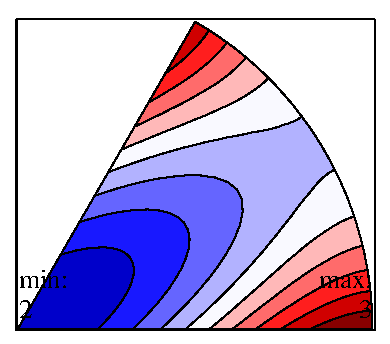
\includegraphics[width=4cm]{pic/tensor1}

      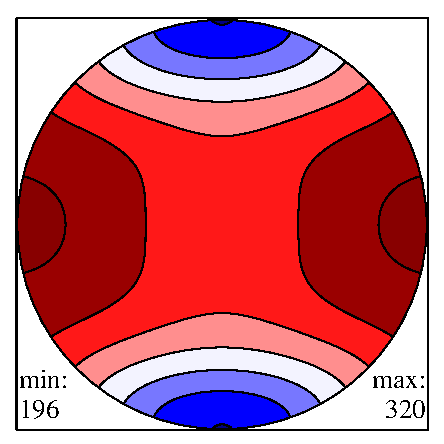
\includegraphics[width=4cm]{pic/tensor}
    \end{column}

  \end{columns}

\end{frame}

\begin{frame}[fragile]
  \frametitle{Field Tensors vs. Matter Tensors}

  \begin{overlayarea}{\textwidth}{\textheight}

  \begin{description}
    \item[field tensors] applied forces, like stress, strain, or a electric
    field
    \item[matter tensors] physical properties like electrical or thermal
    conductivity, magnetic permeability, etc., of a crystalline specimen
  \end{description}

  \begin{onlyenv}<2->
    \begin{lstlisting}[style=input]
S = symmetry('triclinic','mineral','Talc');
\end{lstlisting}
\vspace{-0.3cm}
  \end{onlyenv}

\begin{onlyenv}<3>
  \begin{lstlisting}[style=input]
M = [[219.8  59.6  -4.8 -0.8 -33.8 -1.0];...
     [ 59.6 216.3  -3.6  1.7 -16.5 -0.6];...
     [ -4.8  -3.6  48.8  4.1 -15.5 -3.5];...
     [ -0.8   1.7   4.1 26.5  -3.6 -6.4];...
     [-33.8 -16.5 -15.5 -3.6  22.8 -1.6];...
     [ -1.0  -0.6  -3.5 -6.4  -1.6 78.2]];

C = tensor(M,'name','stiffness','unit','GPa',S)
  \end{lstlisting}
\end{onlyenv}
\begin{onlyenv}<4->
\begin{lstlisting}[style=input]
C = tensor(M,'name','stiffness','unit','GPa',S)
\end{lstlisting}
\vspace{-0.3cm}
\end{onlyenv}
\begin{onlyenv}<4>
\begin{lstlisting}[style=output]
C = elastic stiffness /+tensor+/
     unit: GPa
     rank: 4 (3 x 3 x 3 x 3)
  mineral: Talc (triclinic, X||a*, Z||c)

  tensor in Voigt matrix representation
  219.83    59.66   -4.82  -0.82  -33.87   -1.04
   59.66   216.38   -3.67   1.79  -16.51   -0.62
   -4.82    -3.67   48.89   4.12  -15.52   -3.59
   -0.82     1.79    4.12  26.54   -3.60   -6.41
  -33.87   -16.51  -15.52  -3.60   22.85   -1.67
   -1.04    -0.62   -3.59  -6.41   -1.67   78.29
\end{lstlisting}
\end{onlyenv}

\bigskip

\begin{onlyenv}<5->
import a tensor from the \emph{Material Properties Open Database}

\vspace{-0.2cm}
\begin{lstlisting}[style=input]
T = loadTensor('1000055.mpod')
\end{lstlisting}

\end{onlyenv}

  \end{overlayarea}


\end{frame}




\section{Average Tensors}
\label{sec:average-tensors}

\begin{frame}[fragile]
  \frametitle{Rotating Tensors}

  the orientation of a certain crystal
  \begin{lstlisting}[style=input]
R = orientation('Euler',10*degree,20*degree,0,S)
  \end{lstlisting}

\medskip
\pause

the elastic stiffness tensor in specimen coordinates
\begin{lstlisting}[style=input]
C_rotated = rotate(C,g)
\end{lstlisting}
  \vspace{-.3cm}
\begin{lstlisting}[style=output]
C_rotated = stiffness /+tensor+/
  unit: GPa
  rank: 4 (3 x 3 x 3 x 3)

  tensor in Voigt matrix representation
  228.7  56.0   1.9 19.9 -13.8  6.8
   56.0 176.0  11.6 50.3  -7.6  4.4
    1.9  11.6  43.2  5.2 -19.4  2.3
   19.9  50.3   5.2 43.4  -1.7  0.2
  -13.8  -7.6 -19.4 -1.7  29.3 17.3
    6.8   4.4   2.3  0.2  17.3  73.
\end{lstlisting}



\end{frame}


\begin{frame}[fragile]
  \frametitle{Average Tensors}

The average tensorial property of a specimen can be computed as the average of
the rotated matter tensors of each grain.

\medskip
\pause

The Voigt and the Reuss averages of a tensor $T$ are defines as
\begin{equation*}
  \left<T\right>^{\text{Voigt}}
  = \sum_{m=1}^{M} V_{m} T(g_{m}^{c}), \quad
  \left<T\right>^{\text{Reuss}}
  = \left[ \sum_{m=1}^{M} V_{m} T^{-1}(g_{m}^{c}) \right]^{-1}.
\end{equation*}

\medskip
\pause

For EBSD data this is computed by
\begin{lstlisting}[style=input]
Tmean = calcTensor(ebsd,T,'Voigt')
\end{lstlisting}

\medskip
\pause

and for an ODF by
\begin{lstlisting}[style=input]
Tmean = calcTensor(odf,T,'Voigt')
\end{lstlisting}

\end{frame}

\section{Elastic Deformation}
\label{sec:elasticity}

\begin{frame}[fragile]
  \frametitle{Elasticity Tensors}

  \begin{overlayarea}{\textwidth}{\textheight}

elastic compliance $S$ vs. elastic stiffness $C$
  \begin{lstlisting}[style=input]
S = inv(C)
  \end{lstlisting}

  \begin{onlyenv}<1>
    \vspace{-0.3cm}
\begin{lstlisting}[style=output]
S = compliance /+tensor+/ (show methods, plot)
  unit   : 1/GPa
  rank   : 4 (3 x 3 x 3 x 3)
  mineral: Talc (triclinic, X||a*, Z||c)

  tensor in Voigt matrix representation: *10^-3
  6.9 -0.8  4.7  0.7  6.5  0.3
 -0.8  5.1  1.4 -0.0  1.7  0.0
  4.7  1.4 30.3 -0.1 14.3  0.9
   0. -0.0 -0.1  9.9  2.1  0.8
  6.5  1.7 14.3  2.1 21.7  0.9
  0.3  0.0  0.9  0.8  0.9  3.3
\end{lstlisting}
\end{onlyenv}

\pause
\medskip

stress $\sigma$ vs. strain $\varepsilon$
  \begin{lstlisting}[style=input]
epsilon = EinsteinSum(S,[-1 -2 1 2],sigma,[-1 -2])
  \end{lstlisting}

  \begin{onlyenv}<2>
    \vspace{-0.3cm}
\begin{lstlisting}[style=output]
S = strain /+tensor+/ (show methods, plot)
  rank   : 2 (3 x 3)
  mineral: Talc (triclinic, X||a*, Z||c)

    423   -9.6 -102.9
   -9.6  530.1    8.4
 -102.9    8.4   66.9
\end{lstlisting}
\end{onlyenv}

\pause
\medskip

\begin{onlyenv}<3->

  \begin{columns}
    \begin{column}{7.7cm}

      derived elastic properties
\begin{lstlisting}[style=input]
beta = volumeCompressibility(C)
beta = linearCompressibility(C,x)
E    = YoungsModulus(C,x)
G    = shearModulus(C,h,u)
nu   = PoissonRatio(C,x,y)
T    = ChristoffelTensor(C,n)
\end{lstlisting}


\begin{lstlisting}[style=input]
plot(C,'PlotType',YoungsModulus')
\end{lstlisting}

    \end{column}
    \begin{column}{4cm}
      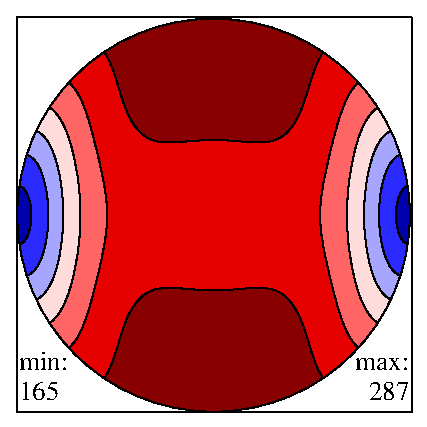
\includegraphics[width=4cm]{pic/YM}
    \end{column}
  \end{columns}
\end{onlyenv}

\end{overlayarea}
\end{frame}


\begin{frame}[fragile]
  \frametitle{Wave Velocities}

\begin{lstlisting}[style=input]
[vp,vs1,vs2,pp,ps1,ps2] = velocity(C,xvector,rho)
\end{lstlisting}

  \begin{columns}
  \begin{column}{8.5cm}

\begin{lstlisting}[style=input]
plot(C,'PlotType','velocity','vp')

hold on
plot(C,'PlotType','velocity','pp')
hold off
\end{lstlisting}

\bigskip
\pause

    \begin{lstlisting}[style=input]
plot(C,'PlotType','velocity','vs1-vs2')

hold on
plot(C,'PlotType','velocity','ps1')
hold off
\end{lstlisting}

  \end{column}
    \begin{column}{3.5cm}
      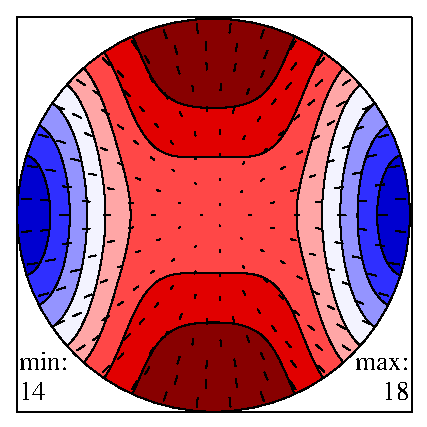
\includegraphics[width=3.5cm]{pic/vp-pp}

      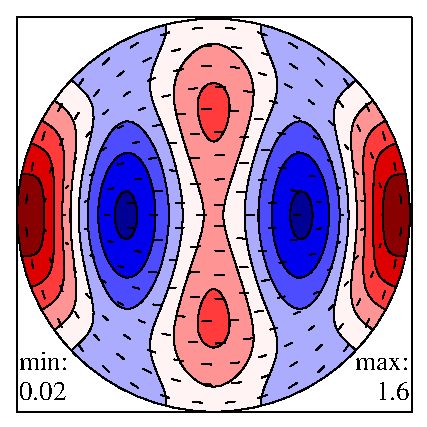
\includegraphics[width=3.5cm]{pic/vs12-ps1}
  \end{column}

  \end{columns}

\end{frame}

\section{Plastic Deformation}
\label{sec:plastic-deformation}

\begin{frame}[fragile]
  \frametitle{Schmidt Factor}

  Consider the slip system
  \begin{lstlisting}[style=input]
b = Miller(0,-1,1,cs,'uvw');  % slip direction
n = Miller(1,1,1,cs,'hkl');   % slip plane normal
\end{lstlisting}

\pause

and the extension direction
  \begin{lstlisting}[style=input]
r = vector3d(0,0,1)           % extension direction
\end{lstlisting}

\pause

\medskip

Then the Schmid factor in direction $\mathbf r$ is given by
\begin{equation*}
  SF = \cos \theta \cos \rho
\end{equation*}

\pause

In \MTEX this can be computed by
  \begin{lstlisting}[style=input]
SF = dot(n,r) * dot(b,r)
  \end{lstlisting}

\end{frame}


\begin{frame}[fragile]
  \frametitle{The Schmid Tensor}

  \begin{overlayarea}{\textwidth}{7cm}
      In tensor language the slip system may expressed as
\begin{lstlisting}[style=input]
ST = SchmidTensor(n,b)
\end{lstlisting}
    \begin{onlyenv}<1>
      \vspace{-0.3cm}
      \begin{lstlisting}[style=output]
ans = symmetric Schmid /+tensor+/
  rank: 2 (3 x 3)

  0   0.5 0
  0.5 0   0
  0   0   0
      \end{lstlisting}
    \end{onlyenv}

\medskip

    \begin{onlyenv}<2-3>
    and the force to the specimen can be described by a stress tensor, e.g.
  \begin{lstlisting}[style=input]
sigma = tensor(
 [[ 0.0 0.0 0.0 ];...
  [ 0.0 0.0 0.0 ];...
  [ 0.0 0.0 1.0 ]],'name','stress');
\end{lstlisting}
    \end{onlyenv}
    \begin{onlyenv}<3>

      \bigskip

Then the Schmid factor is
\begin{lstlisting}[style=input]
SF = EinsteinSum(ST,[-1,-2],sigma,[-1,-2])
\end{lstlisting}
\end{onlyenv}

  \begin{columns}
    \begin{column}{7cm}
      \begin{onlyenv}<4->
  We can do this also for a list of directions
\begin{lstlisting}[style=input]
r = S2Grid('plot','north')
\end{lstlisting}
\end{onlyenv}
      \begin{onlyenv}<5>
        \vspace{-0.3cm}
\begin{lstlisting}[style=output]
r = /+S2Grid+/ (show methods, plot)
  size: 145 x 37
  options: INDEXED, plot, north
\end{lstlisting}
\end{onlyenv}

      \begin{onlyenv}<6->
        \begin{lstlisting}[style=input]
sigma = EinsteinSum(...
         tensor(r),1,...
         tensor(r),2)
       \end{lstlisting}
     \end{onlyenv}
      \begin{onlyenv}<6>
        \vspace{-0.3cm}
\begin{lstlisting}[style=output]
sigma = /+tensor+/ (show methods, plot)
  size: 5365 x 1
  rank: 2 (3 x 3)
\end{lstlisting}
\end{onlyenv}

      \begin{onlyenv}<7->
 \begin{lstlisting}[style=input]
SF = EinsteinSum(...
     ST,[-1,-2],sigma,[-1,-2])

contourf(r,double(SF))
\end{lstlisting}
\end{onlyenv}

    \end{column}
    \begin{column}{5cm}
      \only<7>{
      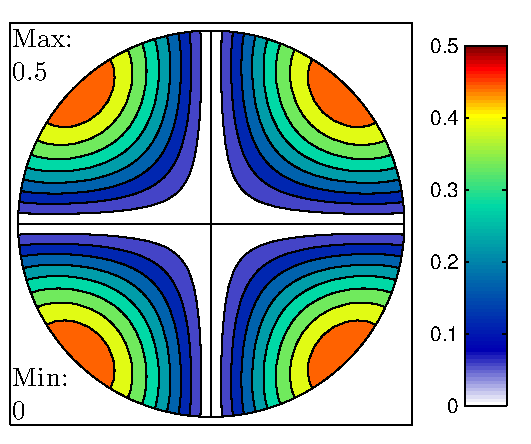
\includegraphics[width=5cm]{pic/SF.pdf}
      }
    \end{column}
  \end{columns}


  \end{overlayarea}

\end{frame}

% \begin{frame}[fragile]
%   \frametitle{Finding the Active Slip Systems}

% Usually there is more the one slip system in a crystal
% \begin{lstlisting}[style=input]
% [bSym,l] = symmetrise(b,'antipodal');
% [nSym,l] = symmetrise(n,'antipodal');

% % restrict b and n to pairs of orthogonal vectors
% [row,col] = find(isnull(...
%   dot_outer(vector3d(bSym),vector3d(nSym))));
% bSym = bSym(row)
% nSym = nSym(col)

% % list of Schmid tensors - one for each slip system
% ST = SchmidTensor(bSym,nSym)

% % list Schmid factors - one for each slip system
% SF = EinsteinSum(RSym,[-1,-2],sigma,[-1,-2])
% [SchmidMax,ind] = max(double(SF))
% \end{lstlisting}


% \end{frame}


\begin{frame}[fragile]
  \frametitle{Finding the Active Slip Systems - Shortcut}

  \begin{columns}
    \begin{column}{7cm}
      Usually there is more the one slip system in a crystal.

      The maximum Schmid factor can be computed by a single command
  \begin{lstlisting}[style=input]
[SFMax,n,b,tau,ind] = ...
  calcShearStress(sigma,n,b)
  \end{lstlisting}

  \bigskip
  \pause

  As usual it is applicable to a list of stress tensors
  \begin{lstlisting}[style=input]
contourf(r,SFMax);
colorbar
  \end{lstlisting}
    \end{column}
    \begin{column}{4cm}
      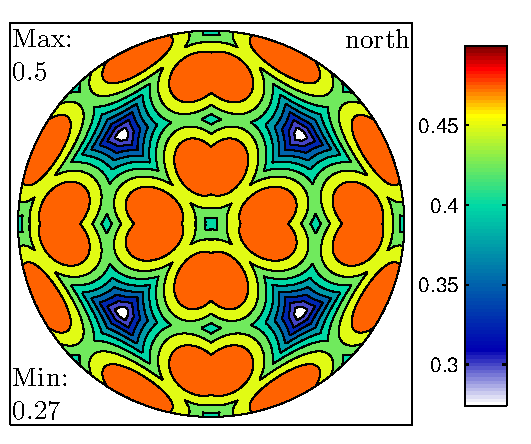
\includegraphics[height=3.5cm]{pic/SFMax}

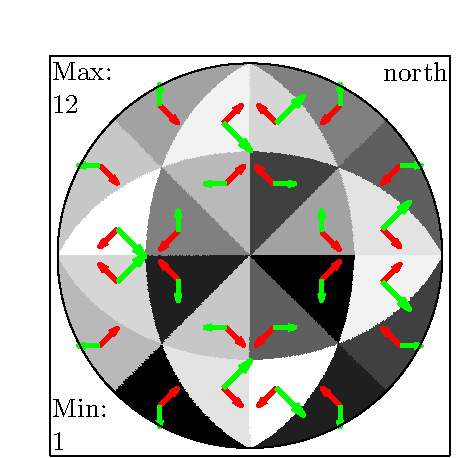
\includegraphics[height=3.5cm]{pic/SFActive}
\end{column}
  \end{columns}


\end{frame}

\begin{frame}[fragile]
  \frametitle{Schmidfactor for EBSD maps}

    \begin{overlayarea}{\textwidth}{\textheight}
    \begin{onlyenv}<1->
      \vspace{-.5cm}
  \begin{lstlisting}[style=input]
ori = get(ebsd('Forsterite'),'orientations')
  \end{lstlisting}
  \vspace{-.3cm}
\end{onlyenv}
\begin{onlyenv}<1>
  \begin{lstlisting}[style=output]
ori = /+orientation+/ (show methods, plot)
  size: 152345 x 1
  crystal symmetry: Forsterite (mmm)
  sample symmetry : triclinic
  \end{lstlisting}
  \end{onlyenv}

  \begin{onlyenv}<2->
  \begin{lstlisting}[style=input]
sigmaCS = rotate(sigma001,inverse(ori))
  \end{lstlisting}
  \vspace{-.3cm}
\end{onlyenv}
\begin{onlyenv}<2>
  \begin{lstlisting}[style=output]
sigmaCS = tensor (show methods, plot)
  size   : 152345 x 1
  rank   : 2 (3 x 3)
  mineral: Forsterite (mmm)
  \end{lstlisting}
\end{onlyenv}
  \begin{onlyenv}<3->
\begin{lstlisting}[style=input]
[SFMax,bActive,nActive,tau,ind] = ...
  calcShearStress(sigmaCS,n,b,'symmetrise');
  \end{lstlisting}
  \vspace{-.3cm}
\end{onlyenv}
\begin{onlyenv}<4->
  \begin{lstlisting}[style=input]
plot(ebsd('Forsterite'),'property',SFMax)
  \end{lstlisting}
\end{onlyenv}

  \begin{onlyenv}<4->
    \centerline{
    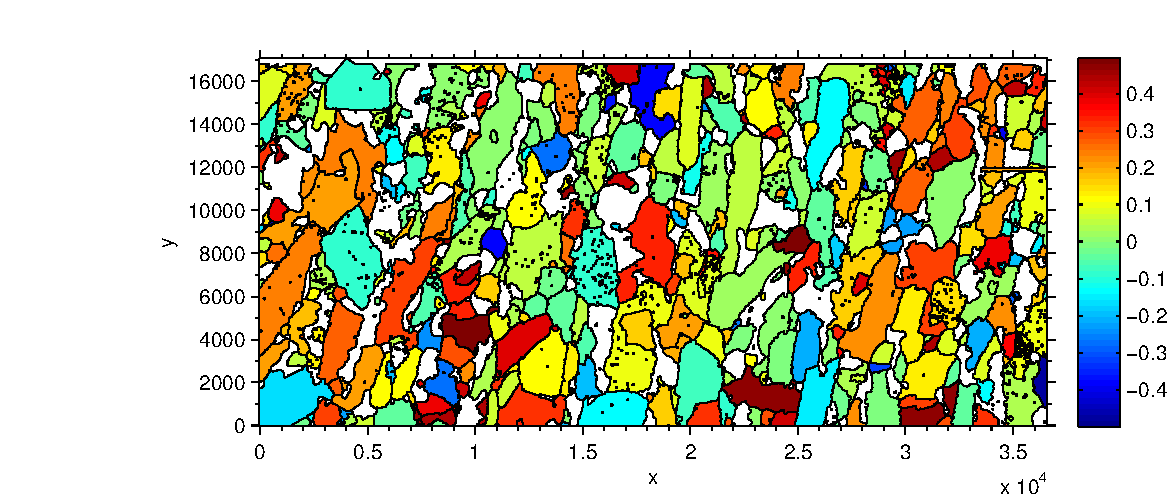
\includegraphics[height=5cm]{pic/SFEBSD.pdf}}
\end{onlyenv}

\end{overlayarea}

\end{frame}



% % The above procedure may also be applied to grains which has the advantage
% % to be much less computational demanding for large data sets.
% %
% % compute grains
% grains = calcGrains(ebsd)

% % extract the orientations
% ori = get(grains('Fe'),'orientation');

% % transform the stress tensor from specimen to crystal coordinates
% sigmaCS = rotate(sigma001,inverse(ori))

% % compute maximum Schmid factor and active slip system
% [Schmid_Max,bActive,nActive,tau,ind] = calcShearStress(sigmaCS,n,b,'symmetrise');

% plot(grains('Fe'),'property',Schmid_Max)
% colorbar



% \begin{frame}
%



% % we observe that the Schmid factor is always between -0.5 and 0.5.
% % The largest value indicates the active slip system.
% % In the above case this would be the slip system found by ind
% Active_Slip_Direction = bSym(ind)
% Active_Slip_Plane = nSym(ind)

% %% Finding the active slip system
% %
% % All the above steps for finding the active slip system,
% % i.e.
% % * find all symmetrically equivalent slip systems
% % * compute all the Schmid factors
% % * find the maximum Schmid factor find the corresponding slip system
% %
% % can be preformed by the single command calcShearStress
% %
%


% \end{frame}



\end{document}





%% Finding the active slip system
%
% With slip direction b and slip plane n also all crystallographic
% symmetric directions and planes which are orthogonal are valid slip
% systems. Let us determine those equivalent slip systems by
% symmetrising b and n

[bSym,l] = symmetrise(b,'antipodal');
[nSym,l] = symmetrise(n,'antipodal');

% restrict b and n to pairs of orthogonal vectors
[row,col] = find(isnull(dot_outer(vector3d(bSym),vector3d(nSym))));
bSym = bSym(row)
nSym = nSym(col)
%
% vizualize crystallographic symmetric slip systems
plot(bSym,'antipodal')
hold all
plot(nSym)
hold off

%% compute Schmid factors for all these slip systems

% define a stress tensor with normal stress in 001 direction
M = zeros(3);M(3,3) = 1;
sigma001 = tensor(M,'name','stress')

% and rotate it a bit
sigmaRot = rotate(sigma001,rotation('Euler',20*degree,20*degree,-30*degree))

% define a list of Schmid tensors - one for each slip sytem
RSym = SchmidTensor(bSym,nSym)

% compute a list Schmid factors - one for each slip system
Schmid_Factor_List = double(EinsteinSum(RSym,[-1,-2],sigmaRot,[-1,-2],'name','Schmid factor'))
[Schmid_Max,ind] = max(Schmid_Factor_List)

% we observe that the Schmid factor is always between -0.5 and 0.5.
% The largest value indicates the active slip system.
% In the above case this would be the slip system found by ind
Active_Slip_Direction = bSym(ind)
Active_Slip_Plane = nSym(ind)

%% Finding the active slip system
%
% All the above steps for finding the active slip system,
% i.e.
% * find all symmetrically equivalent slip systems
% * compute all the Schmid factors
% * find the maximum Schmid factor find the corresponding slip system
%
% can be preformed by the single command calcShearStress
%
[Schmid_Max,bActive,nActive,tau,ind] = calcShearStress(sigmaRot,n,b,'symmetrise')

%%
% This command allows also to compute the maximum Schmidt factor
% and the active slip system for a list of stress tensors in parallel.
% Consider again the list of normal stress tensors corresponding
% to any direction sigma

sigma

% Then we can compute the maximum Schmid factor and
% the active slip system for all these stress tensors by the single command
[Schmid_Max,bActive,nActive,tau,ind] = calcShearStress(sigma,n,b,'symmetrise');

%%
% plot the maximum Schmid factor
contourf(r,Schmid_Max);
colorbar

%% Plot the index of the active slip system

pcolor(r,ind)
mtexColorMap black2white

% We can even visualize the active slip system
% take as directions the centers of the fundamental regions
r = S2Grid(symmetrise([Miller(1,3,5,cs),Miller(-1,3,5,cs)]));

% generate stress tensors
sigma = EinsteinSum(tensor(r),1,r,2)
%sigma = EinsteinSum(tensor(r),1,tensor(r),2) ?

% compute active slip system
[tauMax,bActive,nActive] = calcShearStress(sigma,n,b,'symmetrise');

hold on
% plot active slip plane in red
quiver(r,bActive,'ArrowSize',0.2,'LineWidth',2,'Color','r');

% plot active slip direction in green
quiver(r,nActive,'ArrowSize',0.2,'LineWidth',2,'Color','g');
hold off

%% Real situation in an EBSD map
% So far we have always assumed that the stress tensor is already given
% relatively to the crystal coordinate system. Next we want to examine
% the case where the stress is given in specimen coordinates and
% we know the orientation of the crystal.
% Lets assume we have normal stress tensor in 001 direction
M = zeros(3);M(3,3) = 1;
sigma001 = tensor(M,'name','stress')
%
% Furthermore, we assume the orientations to be given by an EBSD map.
% Thus the next step is to extract the orientations from the EBSD data
% and transform the stress tensor from specimen to crystal coordinates
%
% load MTEX dataset aachen
mtexdata aachen

% extract the orientations
ori = get(ebsd('Fe'),'orientations');

% transform the stress tensor from specimen to crystal coordinates
sigmaCS = rotate(sigma001,inverse(ori))

% Next we compute maximum Schmid factor and the active slip system
% for every orientation in the ebsd data set
[Schmid_Max,bActive,nActive,tau,ind] = calcShearStress(sigmaCS,n,b,'symmetrise');

% plot
plot(ebsd('Fe'),'property',Schmid_Max)
colorbar
%%
% The above procedure may also be applied to grains which has the advantage
% to be much less computational demanding for large data sets.
%
% compute grains
grains = calcGrains(ebsd)

% extract the orientations
ori = get(grains('Fe'),'orientation');

% transform the stress tensor from specimen to crystal coordinates
sigmaCS = rotate(sigma001,inverse(ori))

% compute maximum Schmid factor and active slip system
[Schmid_Max,bActive,nActive,tau,ind] = calcShearStress(sigmaCS,n,b,'symmetrise');

plot(grains('Fe'),'property',Schmid_Max)
colorbar
%% We may also colorize the active slip system.

plot(grains('Fe'),'property',ind)
colorbar
% List slip systems
% extract hkl and uvw values for printing
n_hkl = get(nSym,'hkl');
n_uvw = get(bSym,'uvw');
%
fprintf('  \n')
fprintf('              Slip systems \n')
fprintf('  \n')
fprintf('  #       (hkl)          [uvw]  \n')
for i=1:numel(bSym)
fprintf(' %2i %s %3.0f %3.0f %3.0f %s %3.0f %3.0f %3.0f  \n',i,' ',n_hkl(i,:),'  ',n_uvw(i,:))
end
